\section{Contraposée du théorème de Thalès}
    \subsection{Énoncé}
        \begin{theoreme}[\admis]
            Si dans un triangle $ABC$ :
            \begin{itemize}
                \item $M$ est un point du côté $[AB]$ distinct de $A$ et $B$.
                \item $N$ est un point du côté $[AC]$ distinct de $A$ et $C$.
                \item $\dfrac{AM}{AB} \neq \dfrac{AN}{AC}$.       
            \end{itemize}
            \medskip
            alors les droites $(BC)$ et $(MN)$ ne sont pas parallèles.
        \end{theoreme}

    \subsection{Exemple de rédaction}

        \begin{methode*1}[Justifier que deux droites ne sont pas parallèles]
            \begin{multicols}2
                \begin{itemize}
                    \item Identifier les deux triangles.                                    
                    \item Calculer les rapports de longueurs non portées par les droites candidates.
                    \item Invoquer la contraposée du théorème de Thalès ou le théorème lui-même.
                \end{itemize}
            \end{multicols}

            \exercice

            \begin{minipage}{8cm}
                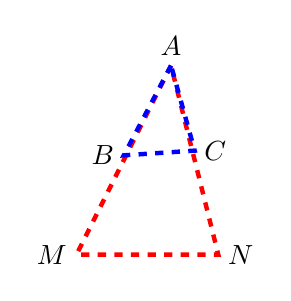
\begin{tikzpicture}[scale = 0.3]
                    % \draw[help lines, color=black!30, dashed] (0,0) grid (12,14);        
                    \coordinate[label=above:$A$] (A) at (7,13);
                    % \coordinate[label=left:$(d')$] (d') at (6.7,14);
                    % \coordinate[label=right:$(d)$] (d) at (7.5,14);
                    \coordinate[label=right:$N$] (N) at (9,5);
                    \coordinate[label=left:$M$] (M) at (3,5);
                    \coordinate[label=left:$B$] (B) at (5,9.2);
                    \coordinate (M1) at (4,5);
                    \coordinate[label=right:$C$] (C) at (8,9.4);
                    \coordinate (N1) at (10,5);
        
                    \tkzDrawSegment(A,M);
                    \tkzDrawSegment(A,N);
                    \tkzDrawSegment(M,N);
                    \tkzDrawSegment(B,C);
                    % \tkzDrawSegment(M1,N1);     
                    \draw[dashed, color=red, ultra thick] (A)--(M)--(N)--(A);
                    \draw[dashed, color=blue, ultra thick] (A)--(B)--(C)--(A);
                \end{tikzpicture}
            \end{minipage}
            \begin{minipage}{8cm}
                \begin{itemize}
                    \item $A$, $B$, $M$ sont alignés.
                    \item $A$, $C$, $N$ sont alignés.
                    \item $AB=\Lg{11.9}$ ; $AM=\Lg{35}$. 
                    \item $AC=\Lg{18.2}$ ; $AN=\Lg{52}$.
                \end{itemize}

                % \vspace*{1cm}
                Démontrer que les droites $(MN)$ et $(BC)$ 
                
                ne sont pas parallèles.
            \end{minipage}
            
            \correction
            Dans le configuration ci-dessus : 
            \begin{itemize}
                \item les deux triangles sont \textcolor{red}{$AMN$} et \textcolor{blue}{$ABC$}.
                \item $B \in [AM]$ et $C \in [AN]$.
                \item D'une part $\dfrac{\textcolor{blue}{AB}}{\textcolor{red}{AM}} = \dfrac{\textcolor{blue}{11,9}}{\textcolor{red}{35}}=0,34$
                \hfill
                D'autre part $\dfrac{\textcolor{blue}{AC}}{\textcolor{red}{AN}} = \dfrac{\textcolor{blue}{18,2}}{\textcolor{red}{52}}=0,35$
            \end{itemize}

            \begin{remarque}
                Les deux rédactions suivantes sont valables.
            \end{remarque}
            
            \hspace*{0.5cm}

            \begin{minipage}{8cm}
                \textbf{or}, si le droites $(MN)$ et $(BC)$ étaient parallèles, d'après le théorème de Thalès, il y aurait égalité des deux rapports
                précédents. Comme ce n'est pas le cas, c'est que \psshadowbox{les droites $(MN)$ et $(BC)$ ne sont pas parallèles}.
    
            \end{minipage}
            \hspace*{0.5cm}
            \vrule
            \hspace*{0.5cm}
            \begin{minipage}{8cm}
                Les rapports précédents étant différents, d'après la contraposée du théorème de Thalès, on peut conclure que \psshadowbox{les droites $(MN)$ et $(BC)$ ne sont pas parallèles}.
            \end{minipage}
        \end{methode*1}
